\documentclass[conference]{IEEEtran}
\IEEEoverridecommandlockouts
% The preceding line is only needed to identify funding in the first footnote. If that is unneeded, please comment it out.
\usepackage{cite}
\usepackage{amsmath,amssymb,amsfonts}
\usepackage{algorithmic}
\usepackage{graphicx}
\usepackage{textcomp}
\usepackage{xcolor}
\usepackage[T1]{fontenc}
\usepackage{lmodern}

\usepackage[justification=centering,skip=10pt,font=footnotesize]{caption}

\DeclareGraphicsExtensions{.pdf,.jpeg,.png,.eps}
\graphicspath{{./eps/}}

\captionsetup{labelsep=newline} % Make a newline between tables and captions

\def\BibTeX{{\rm B\kern-.05em{\sc i\kern-.025em b}\kern-.08em
    T\kern-.1667em\lower.7ex\hbox{E}\kern-.125emX}}
\begin{document}

\title{Blackhole Attack Cooperative Prevention Method in MANETs}

\author{
    Takeru Terai\\
    Ritsumeikan University\\
    Graduate School\\
    of Inf. Sci. Eng.\\
    is0316kf@ed.ritsumei.ac.jp
  \and
    Masami Yoshida\\
    Ritsumeikan University\\
    Graduate School\\
    of Inf. Sci. Eng.\\
    is0195hr@ed.ritsumei.ac.jp
    \and
    Alberto Gallegos Ramonet\\
    Ritsumeikan University\\
    College of\\
    Inf. Sci. Eng.\\
    ramonet@fc.ritsumei.ac.jp
    \and
    Taku Noguchi\\
    Ritsumeikan University\\
    College of\\
    Inf. Sci. Eng.\\
    noguchi@is.ritsumei.ac.jp
}


\maketitle

\begin{abstract}
Blackhole attacks are one of the most serious threats in mobile Ad-hoc networks (MANETs). A blackhole is a security attack in which a malicious node absorbs data packets and sends fake routing information to neighboring nodes. While blackhole attacks are widely studied, existing defense methods wrongfully assume that blackhole attacks cannot overcome the most common defense approaches. This new wave of blackhole attacks is known as smart blackhole attacks. In this study, we use a highly aggressive kind of blackhole attack which is able to predict sequence numbers to overcome the traditional detection methods which set a threshold to sequence numbers. To protect the network from this type of blackhole attack, we propose a detection and prevention method which uses local shared information with neighboring nodes. Our experiments show that our proposed method successfully detects and contain even smart blackhole threats. As a consequence, the attack success rate is decreased.
\end{abstract}

\begin{IEEEkeywords}
AODV, Routing Protocols, MANET, Blackhole, Security
\end{IEEEkeywords}

\section{Introduction}
In recent years, networks that communicate without the use of base stations, such as Ad-hoc networks, have been actively studied. Due to the nature of these networks, their usage is closely related to networks used during natural disasters. In an Ad-hoc network, packets are forwarded to their final destination in a multi-hop fashion; therefore, if there is a malicious node in any relaying node, there is a possibility that an attack such as eavesdropping or data packets falsification may occur \cite{1}. Unlike centralized fixed networks, any node can freely participate in an Ad-hoc network without the existence of an administrator. For this reason, there is an inherent problem with the security of the network. In particular, blackhole attacks (BH attacks) are one of the most serious threats faced by Ad-hoc networks. In BH attacks, an attacking node directs data packets to itself and eavesdrops or discards the packets. When building an Ad-hoc network, it is necessary to ensure reliable security. Therefore, research on defense methods against this type of attack is indispensable in the field of Ad-hoc networks. Although there have been discussions on defense methods for BH attacks, there are few research examples from the perspective of the attacker in BH attacks. When a BH attack uses an unexpected attack pattern, it is necessary to verify whether the existing defense methods can detect and protect from these attacks. In this paper, we propose an aggressive BH attack that can predict the sequence number in the popular Ad-hoc On-Demand Distance Vector (AODV) protocol. We also propose a prevention method that is effective against this attack. We evaluated the performance of this prevention method in terms of packet delivery rate, attack success rate, and false detection rate. Additionally, we demonstrated that the proposed prevention method is effective against BH attacks that can predict the sequence number values.  This paper is organized as follows: Section \ref{aodvSection} describes the functioning of the AODV routing protocol. In Section \ref{bhAttack}, we describe the functioning of a BH attack. Section \ref{blackholeCoop} contains a detailed description of our proposal: the BlackHole Attack Cooperative Prevention Method in mobile Ad-hoc networks(MANETs). Finally, Section \ref{evaluation} presents our evaluations followed by our conclusions.

\section{AODV}
\label{aodvSection}
\subsection{Overview}
AODV \cite{2} is a routing protocol widely used in MANETs. Routing protocols are used to interconnect different points of a network using multiple nodes. A routing table is used in a routing protocol to describe the information of the routes in the network. Protocols that create the routing table can be classified as proactive and reactive. The former is a method in which a routing table is created before the beginning of the communication. The latter does not create routing tables at first but starts creating routing tables when a communication request is issued. AODV belongs to the reactive type and is suitable for creating routes in networks with high node mobility. When determining a route, a sequence number is used. The sequence number is increased when communication is established. If there are multiple route candidates, the route with the larger sequence number is regarded as the newest route and is therefore adopted.

\subsection{AODV route construction}
AODV builds routes by using three types of packets: Route Request (RREQ), Route Reply (RREP), and Route Error (RERR). The information contained in an RREQ and RREP packet is listed in Table \ref{tab:rreqTable} and Table \ref{tab:rrepTable}, respectively. A routing table is created and populated is two steps: 

\textbf{Step 1: RREQ flooding.} Figure \ref{fig:rreqFlooding} shows how RREQ packet flooding works. The source node broadcasts RREQ to its neighboring nodes. The node that receives the RREQ checks whether there is a route to the destination node by consulting its routing table. If there is no route or if the routing table is outdated, it broadcasts the RREQ to its neighboring nodes. This process is performed until the RREQ reaches the destination node or a relay node with an updated route to the destination node.

\textbf{Step 2:  RREP transmission.}  Figure \ref{fig:rrepTrans} illustrates RREP packets transmission. When Step 1 is completed, an RREP is unicasted to the source node that emitted the initial RREQ. These two steps establish a bidirectional path between the source node and the destination node. If the source node receives multiple RREPs, the RREP with the largest sequence number or the smallest number of hops to the target node is adopted.


\begin{table}[h!]
  \begin{minipage}[t]{.45\textwidth}
    \begin{center}
        \caption{RREQ Packet Specification}
        \label{tab:rreqTable}
\begin{tabular}{|c|c|c|}
\hline
Packet Type & Reserved & Hop Count \\
\hline
\multicolumn{3}{|c|}{RREQ ID} \\
\hline
\multicolumn{3}{|c|}{Destination IP Address} \\
\hline
\multicolumn{3}{|c|}{Destination Sequence Number} \\
\hline
\multicolumn{3}{|c|}{Source IP Address} \\
\hline
\multicolumn{3}{|c|}{Source Sequence Number} \\
\hline
\end{tabular}
    \end{center}

  \end{minipage}
  \end{table}
  
  \begin{table}[h!]
  \begin{minipage}[t]{.45\textwidth}
    \begin{center}
        \caption{RREP Packet Specification}
        \label{tab:rrepTable}
\begin{tabular}{|c|c|c|}
\hline
Packet Type & Reserved & Hop Count \\
\hline
\multicolumn{3}{|c|}{Destination IP Address} \\
\hline
\multicolumn{3}{|c|}{Destination Sequence Number} \\
\hline
\multicolumn{3}{|c|}{Source IP Address} \\
\hline
\multicolumn{3}{|c|}{Lifetime} \\
\hline
\end{tabular}
    \end{center}

  \end{minipage}
  \end{table}
  
\begin{figure}[!htb]
\centering

\includegraphics[scale=.035]{RREQ}
\caption{RREQ flooding}
\label{fig:rreqFlooding}
\end{figure}

\begin{figure}[!htb]
\centering
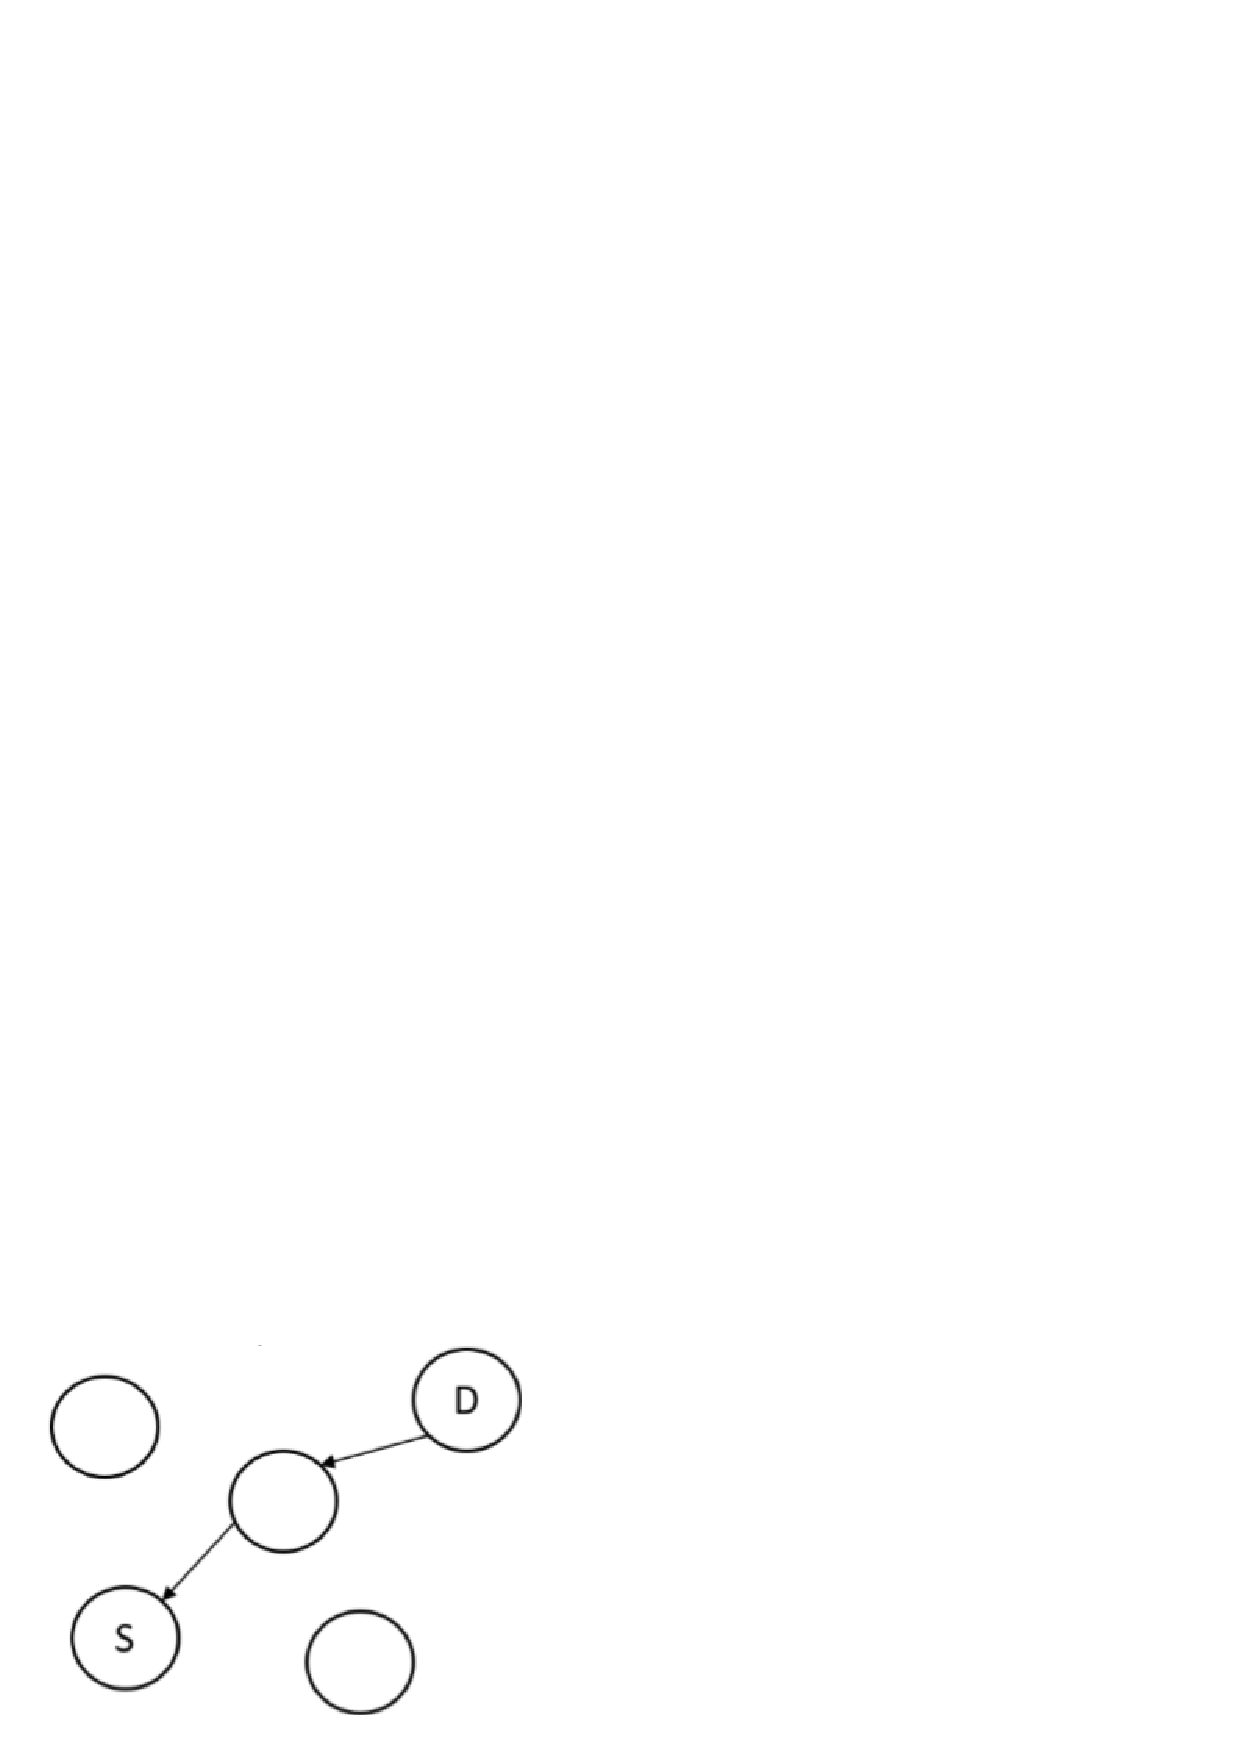
\includegraphics[scale=.60]{RREP}
\caption{RREP transmission}
\label{fig:rrepTrans}
\end{figure}

\section{BH attack}
\label{bhAttack}
\subsection{Overview}
A BH is a type of Denial of Service (DoS) attack that discards or eavesdrops on data packets that are sent from a source node to a destination node \cite{3, 4}. The BH node catches an RREQ and returns an RREP with a spoofed sequence number to the source node, thereby constructing a communication path that includes the BH node. The BH node can disrupt the communication by absorbing the passing packets itself. As a result, the throughput and packet arrival rate decrease dramatically.

\subsection{BH attack procedure}
As previously mentioned, the BH node directs data packets to itself by using spoofed RREPs. Figure \ref{fig:bhAttack} shows this process, where the attacking node is B.

\begin{figure}[htb]
\centering
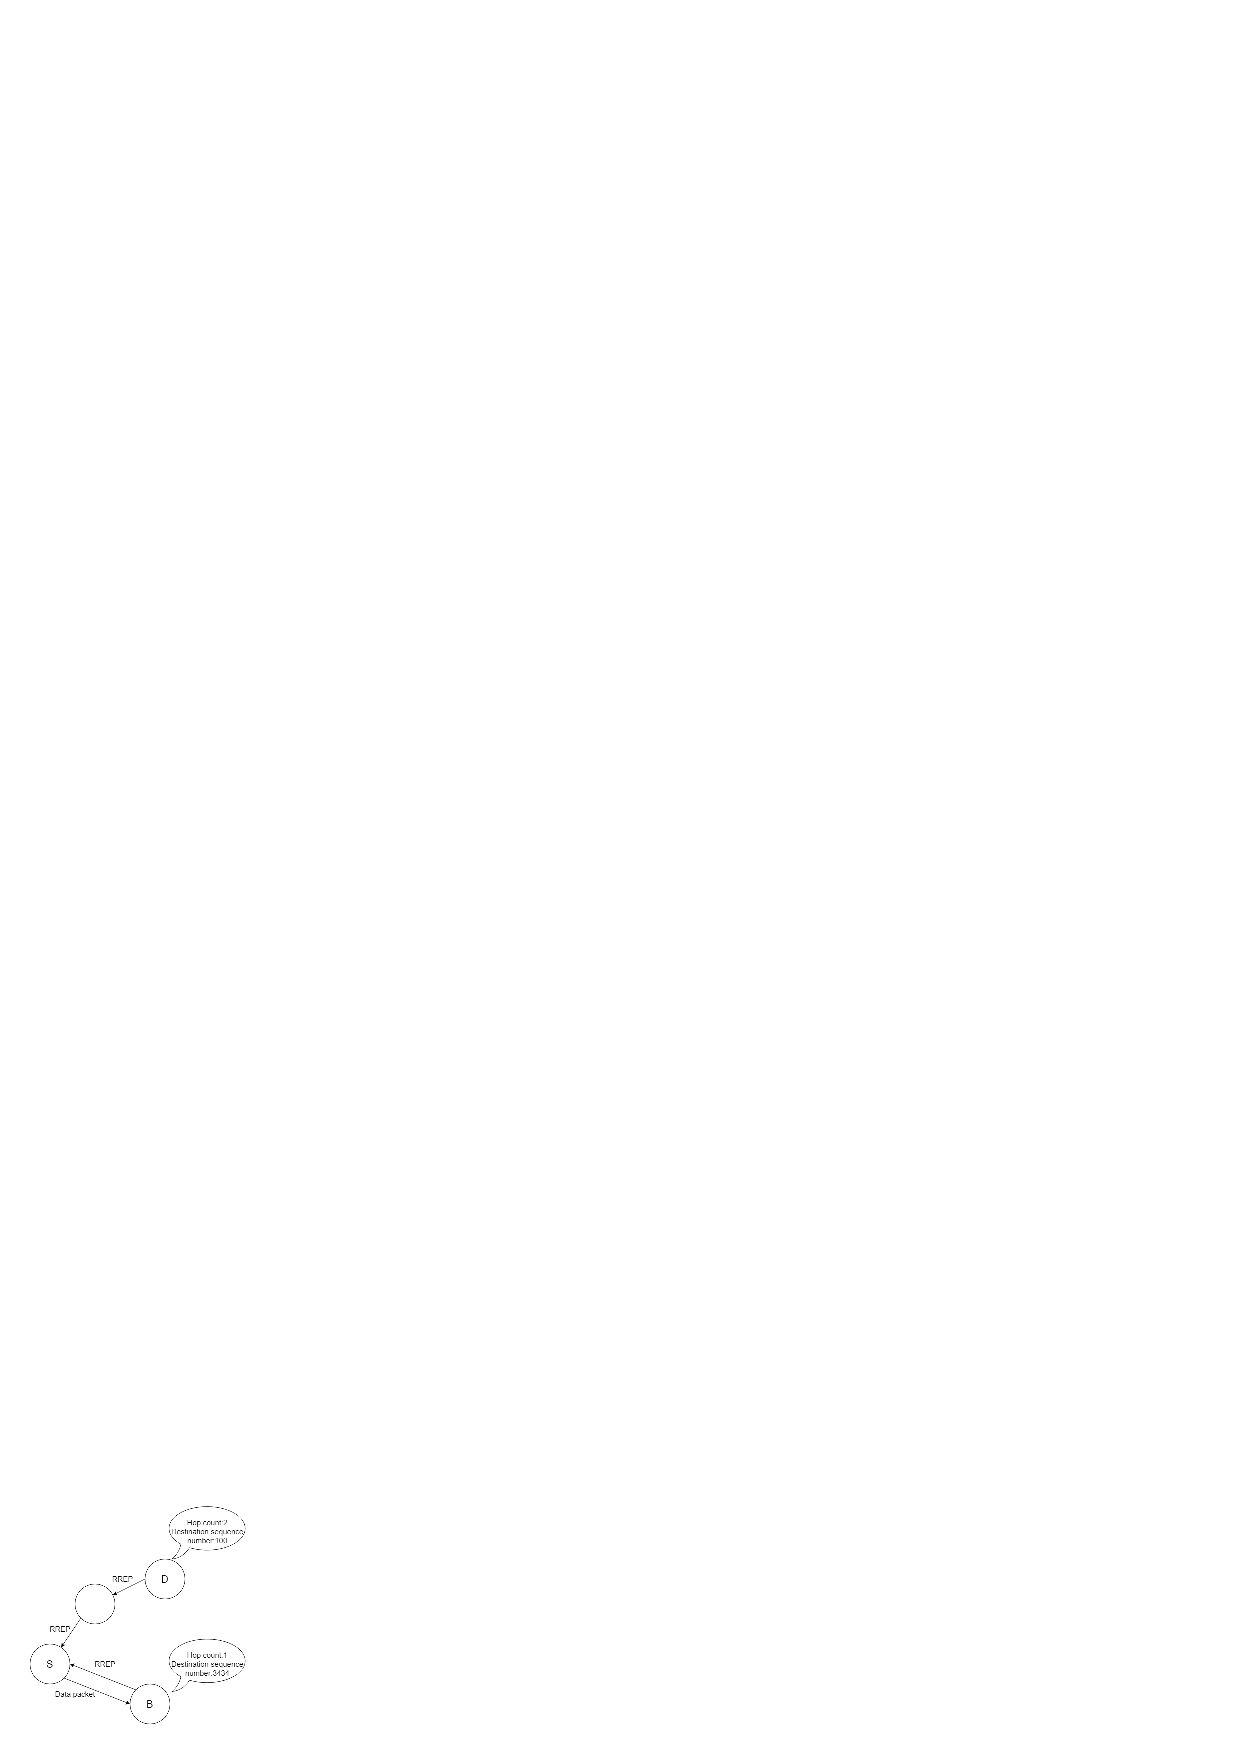
\includegraphics[scale=1.7]{BH_Attack}
\caption{BH Attack}
\label{fig:bhAttack}
\end{figure}


\textbf{Step1: Transmission of a spoofed RREP.} When the BH node receives the RREQ, it sends a spoofed RREP. At this time, the number of hops described in the RREP is set to a small value, and the sequence number is set to any value larger than the actual sequence number. By setting the sequence number to a larger value, the BH attack ensures that the path that includes the BH node is considered by the neighboring nodes as the most up to date route.

\textbf{Step 2: Data packet routing.} The source node receives the spoofed RREP from the BH node.  When the source node receives this information, it assumes that this path in which the malicious node exists has the smallest number of hops and is the most up to date path. Therefore, then source node sends the data packets to the malicious node.

\subsection{Existent defense methods and Smart BH attacks}
BH attacks are significant threats in MANETs. A BH attack can degrade the performance of most networks even to the point of invalidating them. For example, some BH defense methods use dummy RREQ \cite{13} to detect the existence of BH nodes. This defense method assumes that a BH node responds to an RREP immediately upon receiving RREQ. Nodes responding to a dummy RREQ with a nonexistent address are considered BH nodes with this defense method. However, smart BH nodes can infer whether the destination address exists to some extent and easily overcome this defense method. Other existent defense methods against BH attacks mainly consist in setting a threshold for sequence numbers \cite{5, 6}.  Typical BH attacks create RREP messages with a large sequence number value. Therefore, simply limiting the sequence numbers can help to protect against these attacks. This kind of defense method is known as \textit{threshold-based defense}. This common defense method is shown in Figure \ref{fig:ThresholdDefense}. In this figure, \mbox{node S} sets the sequence number threshold to 1000. Because the destination sequence number of the RREP created by node D is 100 (which is below the threshold), node S identifies node D as a safe node. On the other hand, the destination sequence number of the RREP created by node B is 3434 (which is larger than the threshold), therefore, node S determines that the destination sequence number of the RREP created by node B is spoofed, identifies the node B as a BH node and discards its subsequent RREPs. However, this defense method does not assume that the BH node can use a sophisticated attack capable of setting sequence numbers intelligently. Smart BH attacks defeat the threshold-based defense methods by taking note of the destination node sequence numbers of the received RREQ and predicting the actual sequence number values to some extent using the least-squares method (dynamic threshold attack) \cite{8,3}. It is not unreasonable to assume that smart BH attacks can overcome most defense methods that use a similar approach as threshold-based defense methods. For example, the method proposed in \cite{7} achieves a high packet delivery rate even with the existence of regular BH attacks. According to the authors, this is possible by creating a threshold which is set as a small amount above the average of all received RREPs. However, this method does not consider smart BH attacks, and therefore, it is ineffective against attacks that predict sequence numbers. Multiple studies \cite{10,11,12} are effective against regular BH attacks but pale when proved against smart BH attacks. Security is an indispensable part of WSN, and defense methods should be capable of detecting and preventing BH attacks even when attacks are capable of predicting sequence numbers.  In this paper, we created a smart BH attack and propose a defense method against it. Additionally, we show the effectiveness of this smart BH attack when traditional BH defense methods are used. In our evaluations, we used the common \textit{threshold defense} method to demonstrate the effectiveness of the smart BH attack. Our original defense method proposal is capable of dealing with smart BH attacks. This proposal uses the cooperation of neighboring nodes to set even more suitable sequence numbers thresholds. 
 
\begin{figure}[!htb]
\centering
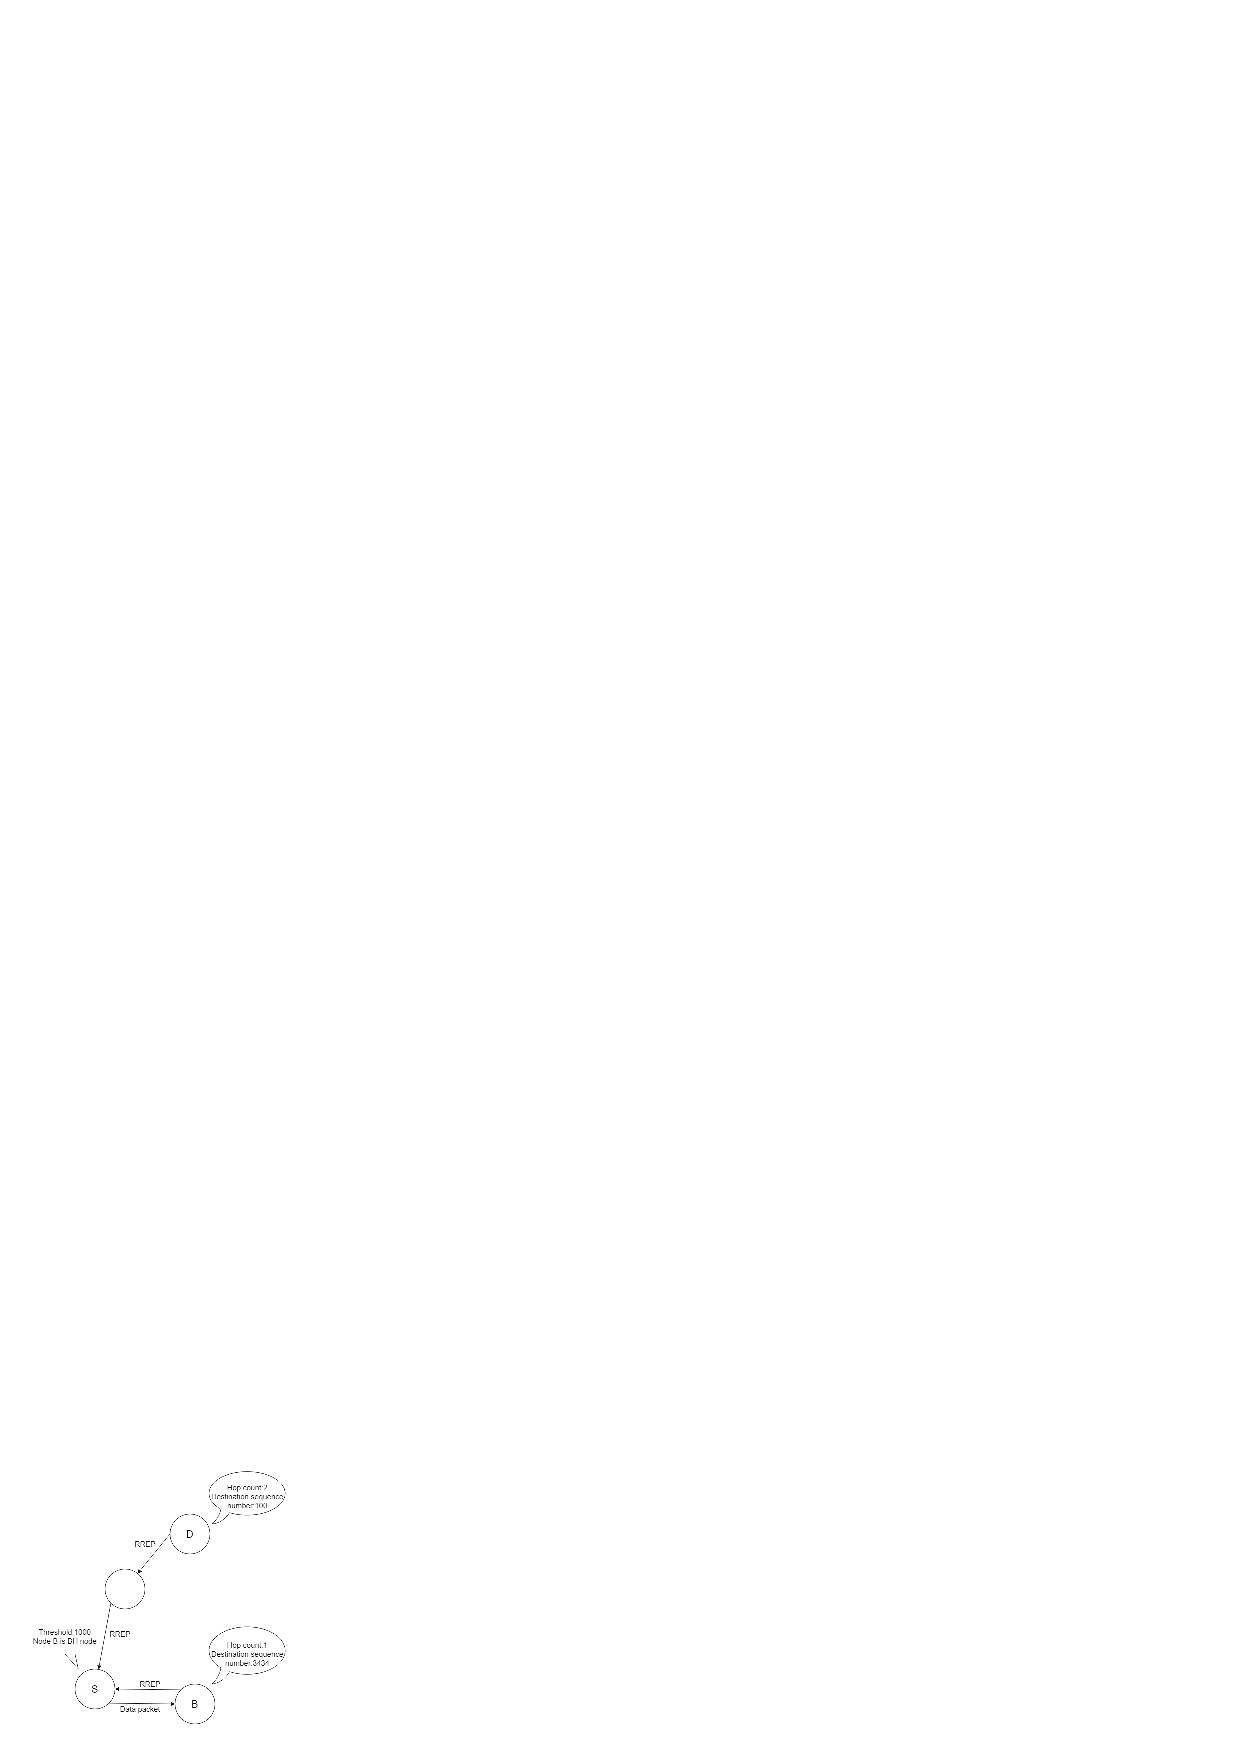
\includegraphics[scale=1.6]{Threshold_Defense_Method}
\caption{Threshold Defense Method}
\label{fig:ThresholdDefense}
\end{figure} 
\section{Blackhole Attack Cooperative Prevention Method}
\label{blackholeCoop}


\subsection{Overview}
Our proposed defense method uses the sequence number and creation time (timestamp) described by the RREPs coming from the destination node. The sequence number is predicted using the least-squares method to set the threshold value. To improve the approximation accuracy, the source node shares the sequence number and the timestamp information with its neighboring nodes. The node that transmitted the RREQ is the only node that can detect the BH node. A flow chart of the defense method is shown in \mbox{Figure \ref{fig:FlowchartDefense}}.
\begin{figure}[!htb]
\centering
\includegraphics[scale=.5]{The_flowchart_of_defense_method}
\caption{Flowchart of the defense method}
\label{fig:FlowchartDefense}
\end{figure}


\subsection{Obtaining the sequence number and timestamp}
There are two types of acquisition means for sequence numbers and timestamps from the destination node to protect against BH attacks:

\begin{itemize}
  \item Collecting the information contained in an RREP packet coming from the destination node.
  \item Obtaining the information of the destination nodes from neighboring nodes.
\end{itemize}

The first method can be used within the normal operations of the AODV protocol without changing its implementation because a node simply retrieves the destination node address and destination sequence number from the received RREP packet. For the second method, it is necessary to change the implementation of AODV to share information from the neighboring nodes. Part of our proposal in this paper involves this second method. By changing the contents of the RREP packet, it is possible to share information held by the neighboring nodes with the source node. The modified RREP packet is shown in \mbox{Table \ref{tab:modRrep}}. This RREP contains two new elements: {\it Shared Sequence Number} and {\it Creation Time of The RREP packet (TimeStamp)}. A relay node puts the last destination sequence number known by itself into shared sequence number in the RREP. That is, shared sequence number is an item to be written when the sequence number of the destination node was acquired from an RREP received and forwarded in the past. A relay node puts the time of acquiring the sequence number information into the "creation time of the RREP in which the shared sequence number was originally contained (Timestamp)". Therefore, all nodes must hold the destination sequence number value of the RREP received in the past and the timestamp information of the RREP.


  \begin{table}[h]
  \begin{minipage}[t]{.45\textwidth}
    \begin{center}
        \caption{Modified RREP Specification}
        \label{tab:modRrep}
\begin{tabular}{|c|c|c|}
\hline
Packet Type & Reserved & Hop Count \\
\hline
\multicolumn{3}{|c|}{Destination IP Address} \\
\hline
\multicolumn{3}{|c|}{Destination Sequence Number} \\
\hline
\multicolumn{3}{|c|}{Source IP Address} \\
\hline
\multicolumn{3}{|c|}{Lifetime} \\
\hline
\multicolumn{3}{|c|}{Creation Time of The RREP (Timestamp)} \\
\hline
\multicolumn{3}{|c|}{Shared Sequence Number} \\
\hline
\multicolumn{3}{|c|}{\shortstack{Creation Time of The RREP\\ in which the shared sequence number\\ was originally contained (Timestamp)}} \\
\hline
\end{tabular}
    \end{center}

  \end{minipage}
  \end{table}

\subsection{Threshold creation}
\label{thresholdCreation}
The source node predicts the sequence number using the least squares method with its own information and information collected from its neighboring nodes. Through preliminary experiments, we confirmed that the sequence number increased proportionally with the time. Therefore, the least square method involves using two pairs of data: the destination sequence number and the acquisition time of the sequence number. For example, let $T_1, T_2, T_3,...$ be a sequence of acquisition times of a destination sequence number for a given destination IP address and $S_1, S_2, S_3,...$ be the destination sequence numbers corresponding to each acquisition time. With these times, we calculate the elapsed times $X_i$ between reception of the first sequence number and the subsequent sequence numbers $(X_i = T_i - T_1)$. By using these datasets $(X = X_1, X_2, X_3, X_n$ and $Y = S_1, S_2, S_3, S_n)$, it is possible to calculate the equation of a straight line (slope and intercept). The slope and intercept are given by the Equations \ref{eq:slope} and \ref{eq:intercept}, respectively.

\begin{equation}
\label{eq:slope}
slope:A= \frac{Cov (X,Y)}{\sigma^2_X}
\end{equation}

\begin{equation}
\label{eq:intercept}
intercept:B=\overline{Y}-A\overline{X}
\end{equation}

$\overline{X}$ represents the average of $X$, $\sigma_X$ represents the standard deviation of $X$,  $\overline{Y}$ is the average of $Y$, and $COV (X,Y)$ represents the covariance between $X$ and $Y$. For example, suppose that the data sets $(X,Y)$ are (2, 4), (3, 5), (10, 18) and (13, 29). In this case, $x = 7$, $y = 14$, $\sigma_X=\sqrt{\displaystyle \frac{43}{2}}$, $Cov(X,Y)=47$, $slope:A=\displaystyle \frac{94}{43}$ and $intercept:B=\displaystyle -\frac{56}{43}$. Therefore, the standard equation of a line can be derived as $y=\displaystyle \frac{94}{43}x-\displaystyle \frac{56}{43}$. For example, when $x=3$ is substituted into this equation, $y=\displaystyle \frac{226}{43} \approx 5.2558$, which approximately matches the data of (3, 5). With this standard equation, the actual sequence number value is calculated (predicted) at any given time and the threshold can be defined. To decrease the false detection rate, which is the ratio of the number of normal nodes considered falsely as a BH node to the total number of normal nodes, the threshold must be slightly higher than the actual sequence number value. That is, the threshold value is defined by Equation \ref{eq:thresholdValue}.

\begin{equation}
\label{eq:thresholdValue}
TH = Seq_a + \alpha
\end{equation}

TH represents the threshold, $Seq_a$ represents the approximated actual sequence number, and the parameter $\alpha$ is a safety margin for preventing the false detection of a BH node. Depending on the value of $\alpha$, the performance can greatly change. A smaller value of $\alpha$ increases the detection rate of BH nodes but also increases the false detection rate. A larger value of $\alpha$ decreases the false detection rate but also decreases the detection rate of BH nodes. 

\section{Performance evaluation}
\label{evaluation}

\subsection{Simulation environment}
We evaluated the performance of the proposed BH attack defense method using the ns2 network simulator \cite{9}. There are many studies that have used ns2 for research evaluation. The simulation environment is described in Table \ref{tab:simEnviro}. We implemented a smart BH attack and implemented a defense method against this attack. In addition to the proposed defense method in this paper, we also evaluated and compared a BH attack prevention method using a dynamic threshold in MANETs \cite{3}. This method classifies nodes as either normal or BH using a dynamically updating sequence number threshold. The threshold is calculated from the total number of active nodes and the time elapsed from the reception of the last routing control packet. In the evaluation of these methods, the number of nodes was changed from 20 to 50, and the number of trials was set to 30 for each number of nodes. The results are an average of the 30 observations. For $\alpha$ mentioned in Subsection \ref{thresholdCreation}, we set it to the optimal value $\alpha = 4$, which was obtained from preliminary experiments. We evaluated the defense methods from three perspectives: packet delivery rate, attack success rate, and false detection rate \mbox{(Equations \ref{eq:packetDelivery}, \ref{eq:attackSuccess} and \ref{eq:detectionRate})}.

\begin{equation}
\label{eq:packetDelivery}
PDR=\displaystyle \frac{N_{recv}}{N_{sent}} \times 100 
\end{equation}

Packet delivery rate (PDR) represents how much data was sent from the source node to the destination node. $N_{recv}$ is the number of data packets received by destination node and $N_{sent}$ is the number of data packets transmitted by the source node.

\begin{equation}
\label{eq:attackSuccess}
ASR=\displaystyle \frac{{NF}_{selected}}{{NF}_{recv}} \times 100
\end{equation}

Attack success rate (ASR) represents how much the BH node was able to guide data packets to itself against the number of attacks. ${{NF}_{selected}}$ is the number of times a route through a BH node was selected based on the spoofed RREPs of which sequence numbers are smaller than the threshold. ${NF}_{recv}$ is the number of spoofed RREPs created by a BH node received by the source node.

\begin{equation}
\label{eq:detectionRate}
FDR=\displaystyle \frac{{N\_TH}_{over}}{NT_{recv}} \times 100
\end{equation}

False detection rate (FDR) indicates how many normal nodes was treated as a BH nodes. ${N\_TH}_{over}$ is the number of unspoofed RREPs of which sequence numbers are bigger than the threshold. $NT_{recv}$ is the number of unspoofed RREPs created by a normal node received by the source node.

\begin{table}[htbp]
\begin{center}
\caption{Simulation Environment}
\label{tab:simEnviro}
\begin{tabular}{|c||c|}
\hline
Simulation Time & 200[s] \\
\hline
Network Area & 800[m]×800[m] \\
\hline
Number of nodes & 9, 19, 29, 39, 49 \\
\hline
Number of BH nodes & 1 \\
\hline
Mobility model & Random Waypoint \\
\hline
$\alpha$ & 4 \\
\hline
\end{tabular}
\end{center}
\end{table}

Evaluations of ASR and FDR are new evaluations not conducted in our prior work\cite{8}.

\subsection{Evaluation results and considerations}

\subsubsection{Packet delivery rate}
Figure \ref{fig:pdr} shows the results of the packet delivery rate evaluation. As the number of nodes increases, the packet delivery rate tends to increase. This is because stable links could be established as the number of nodes increased. The proposed method shows a higher packet delivery rate than the existing threshold-based method or no protection at all. The packet delivery rate increased by approximately 30\% or more compared to not using the proposed method. However, this number was able to increase up to 40\% as the number of nodes increased. Also, compared with the existing threshold-based method, the packet delivery rate increased by 10\% or more and increased up to 15\% as the number of nodes increased. In the proposed method, the packet delivery rate tends to increase as the number of nodes increases. This is because the increase in the number of nodes allows the node that creates a threshold to obtain more information from its neighboring nodes and therefore accurately predict the destination sequence number.

\begin{figure}[!htb]
\centering
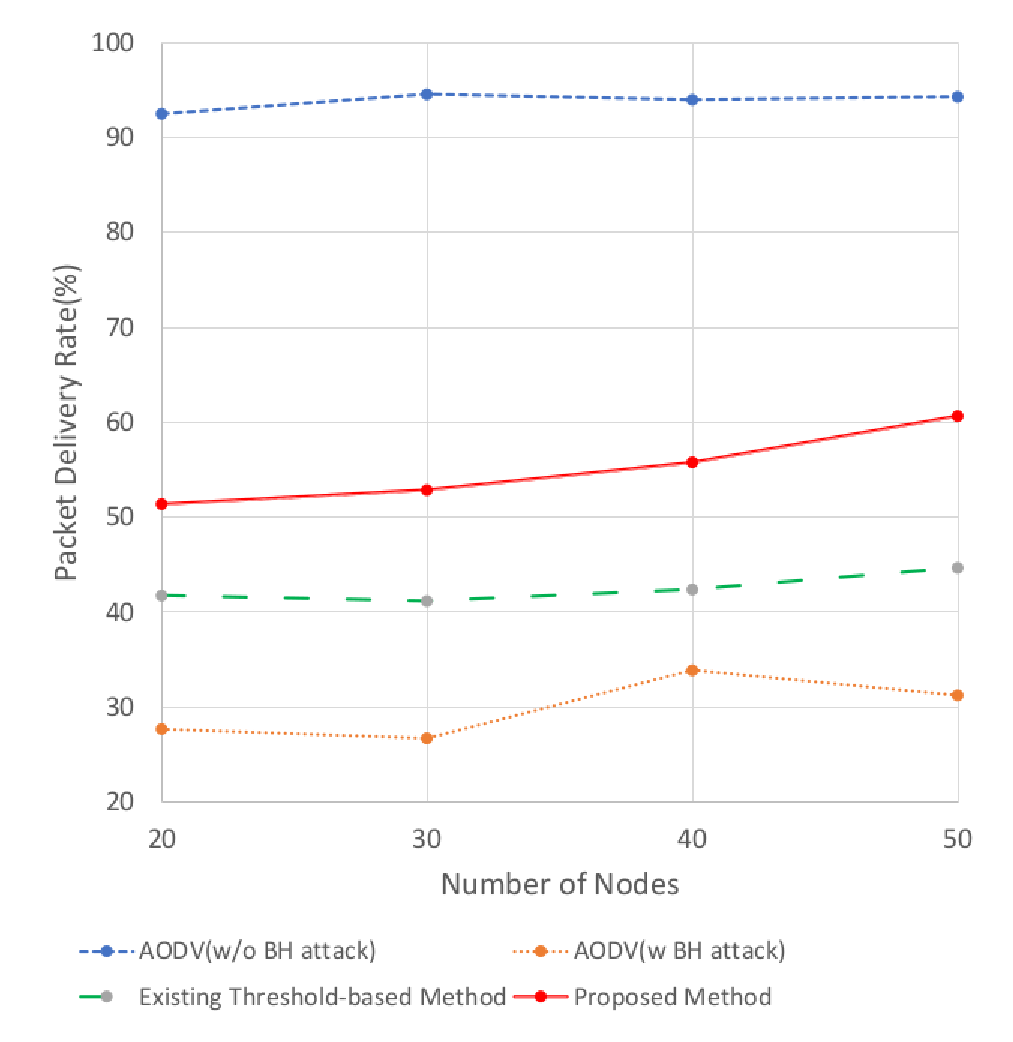
\includegraphics[scale=0.45]{PDR}
\caption{Packet Delivery Rate}
\label{fig:pdr}
\end{figure}

\subsubsection{BH attack success rate}
Figure \ref{fig:attackSuccessRate}  shows the results of the BH attack success rate. When the proposed method was used, the attack success rate was reduced by 50\%. This is because the source node can accurately predict the sequence number and set an appropriate threshold. In comparison, the attack success rate was reduced only by 40\% when using the existing threshold-based method. However, the attack success rate of the proposed method may differ depending on the number of nodes. The attack success rate of the proposed method with 20 nodes was relatively high. This is because the attacking BH node could not deceive the protection with their spoofed sequence numbers. It has been proven that the effectiveness of the BH attack method used in this study decreases as the number of nodes decreases \cite{8}. When the number of nodes is low, there is a high probability that the route where the BH node exists is not selected because the sequence number set by the BH node is too large or too small. The attack success rate is greatly reduced due to this. The attack success rate was the highest for 30 nodes but was greatly reduced using 40 and 50 nodes. This is also because the increase in the number of nodes allows a node to create a more appropriate threshold.


\begin{figure}[!htb]
\centering
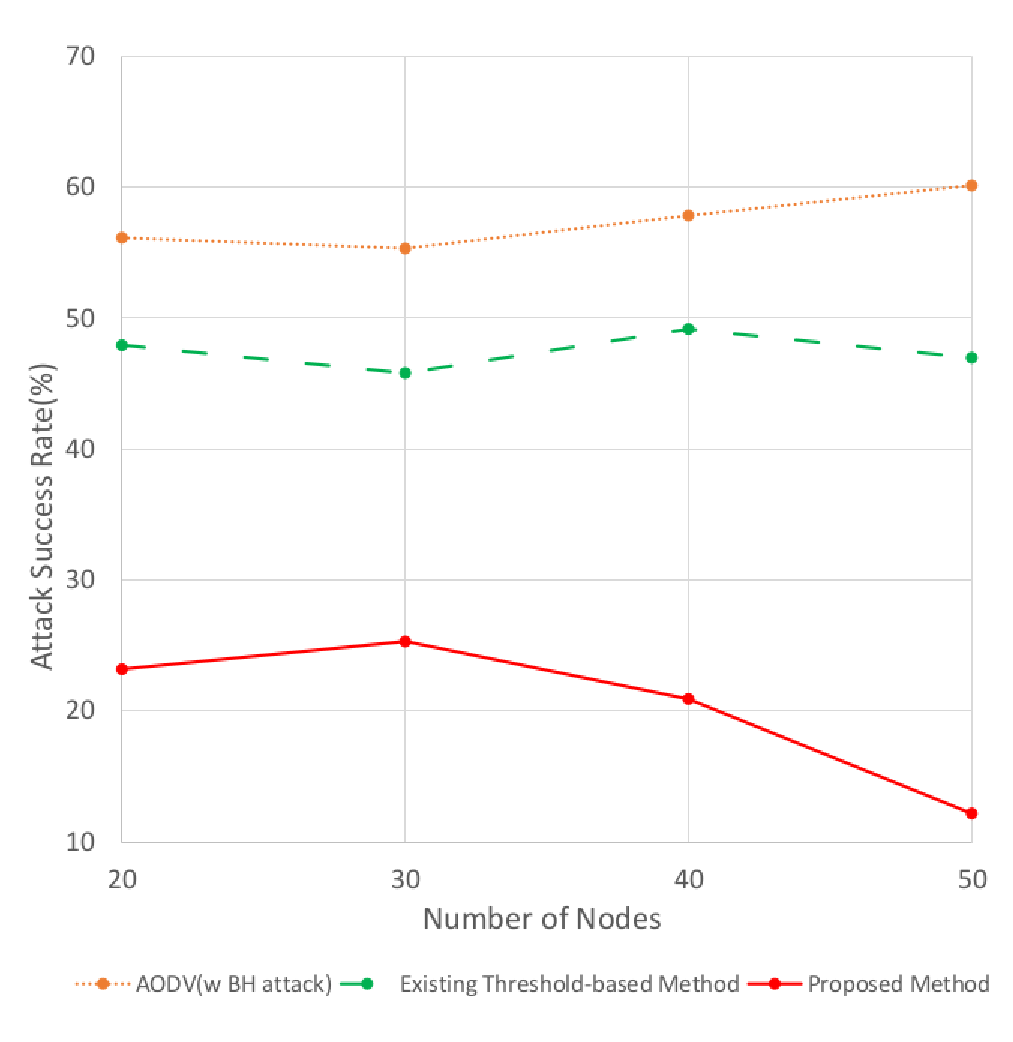
\includegraphics [scale=0.45]{ASR}
\caption{Attack Success Rate}
\label{fig:attackSuccessRate}
\end{figure}

\subsubsection{False detection rate}
Figure \ref{fig:falsePositive} shows the results of false detection rate. The rate decreases with an increase in the number of nodes. This decrease occurs for the same reason as that of the packet delivery rate. However, our results showed that the false detections rate was high when the number of nodes was 20. This is a problem caused by setting the parameter $\alpha$ in the proposed method. The most adequate value of $\alpha$ was determined to be 4 based on prior experiments. This value can greatly differ depending on the number of nodes. We performed several trials for each number of nodes. We found an $\alpha$ value that minimizes the false detections rate in each trial. However, when the number of nodes was small, the variability of each trial was large, and when the number of nodes was large, the adequate value of $\alpha$ was close to 4. The parameter $\alpha$ is also affected by the value of the spoofed sequence number generated by a BH node. When the number of nodes is small, the spoofed sequence numbers set by the BH nodes can also greatly vary. For this reason, the parameter $\alpha$ that minimizes the false detection rate also varies. For example, in our experiments, when the number of nodes was 20, the false detection rate was high. However, as the number of nodes increased, the false detection rate was reduced significantly. The proposed method resulted in a large false detection rate when compared to the existing threshold-based method. In Figure \ref{fig:SuccessAndFalse}, we compare the attack success rate and false detection rate. If the threshold is set to an extremely small value, the BH node can be detected but a normal node can also be erroneously determined as a BH node. If the threshold is set to an extremely large value, an erroneous evaluation is unlikely to occur, but it is difficult to detect BH nodes. Therefore, the greater the sum of the attack success rate and the false detection rate (especially as it approaches 100), the better an attack is prevented but the larger the misjudgment, and vice versa.  Comparing the proposed method and the existing threshold-based method, the sum of the attack success rate and false detection rate is smaller in the proposed method except for with 20 nodes. This can be explained by the fact that the proposed method can set a more accurate threshold value in terms of attack detection and misjudgment.


\begin{figure}[!htb]
\centering
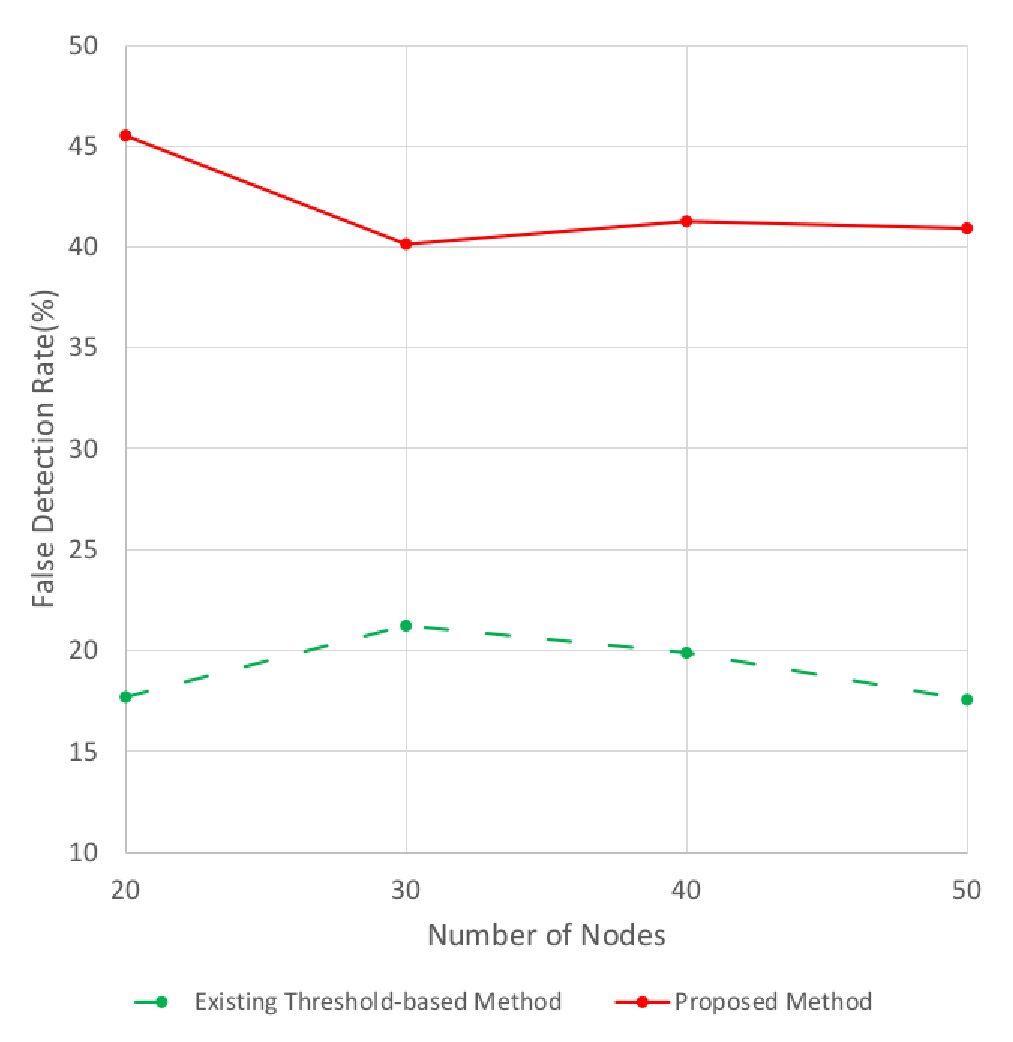
\includegraphics [scale=0.45]{FDR}
\caption{False Detection Rate}
\label{fig:falsePositive}
\end{figure}

\begin{figure}[!htb]
\centering
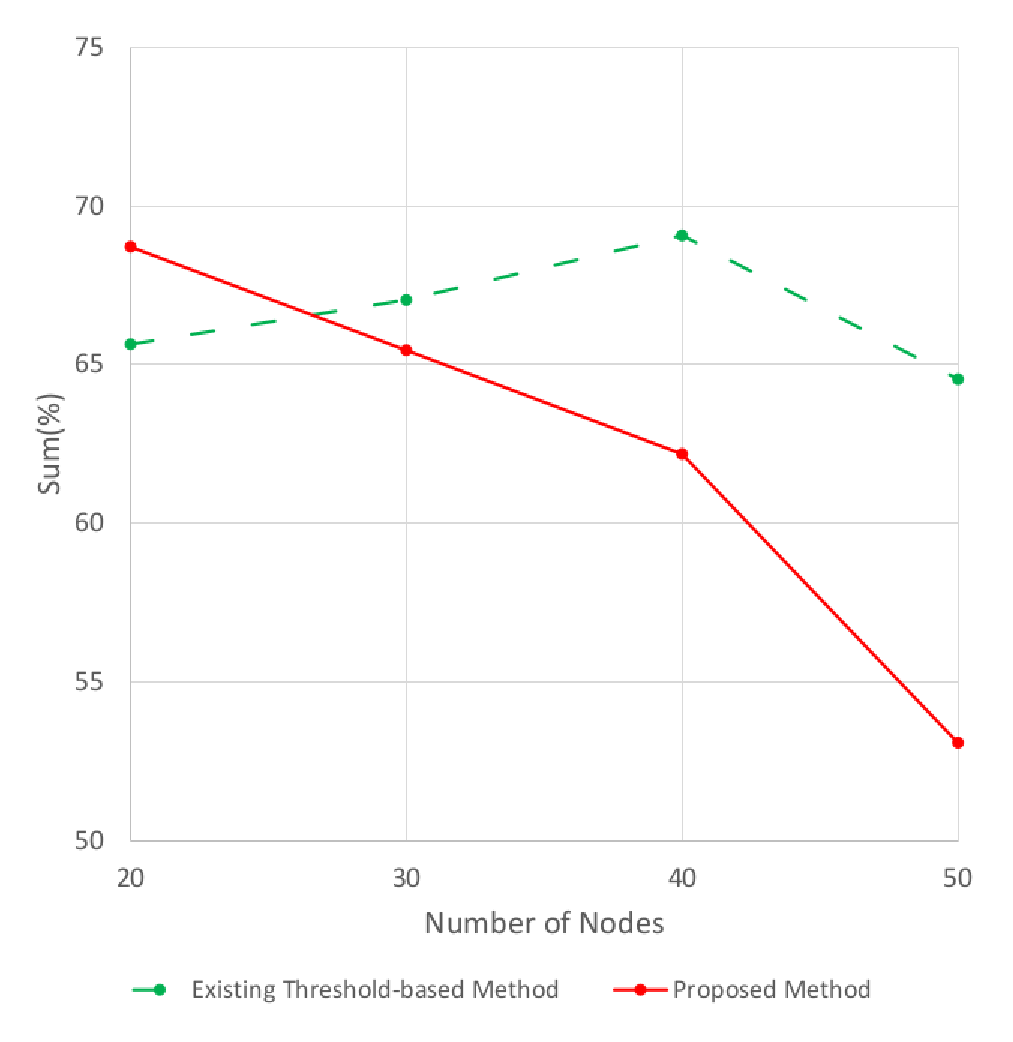
\includegraphics[scale=0.45]{ASRFDR}
\caption{Attack Success Rate and False Detection Rate}
\label{fig:SuccessAndFalse}
\end{figure}

\section{Future work}
In the future, we aim to improve the proposed method and reduce the false detections rate. Future improvements will address this and use an adaptive method that works in every situation. BH nodes present multiple signature behaviors that can be exploited in their detection. For example, a BH node returns an RREP immediately upon receiving an RREQ. This behavior suggests that the BH node is a node that creates more RREPs than other nodes. This can be exploited in early BH attacks detection. In our future work, analysis of such behaviors will be used to detect and defend from ingenious BH attacks.

\section{Conclusion}
In this paper, we proposed a defense method that allows nodes to share local information with their neighboring nodes. Furthermore, we aimed at minimizing false detections rate while maintaining the packet delivery rate. In our proposal, we used information from neighboring nodes and created a sequence number threshold based on this information. We evaluated the proposed method using simulations. When the proposed method was applied to existing attack methods, we succeeded in improving the packet delivery rate by up to 40\% and reduced the attack success rate by up to 50\%. Also, when compared to the dynamic threshold protection method, we succeeded in increasing the packet delivery rate by up to 15\% and reduced the attack success rate by up to 40\%. Our proposal showed that the cooperation of multiple nodes can improve the accuracy of the nodes' sequence numbers threshold approximations and therefore, improve the overall detection process when compared to traditional BH detection methods which cannot detect a smart BH attack. To reduce the false detection rate, we will improve the proposed method.

%\newpage

\bibliographystyle{IEEEtran}
\bibliography{terai}


\end{document}
